%%%%%%%%%%%%%%%%%%%%%%%%%%%%%%%%%%%%%%%%%%%%%%%%%%%%%%
% For this chapter I need to build the figures.
% NOT done yet.
% Also need to be checked, but this will happen after
% the figure insertion.
%%%%%%%%%%%%%%%%%%%%%%%%%%%%%%%%%%%%%%%%%%%%%%%%%%%%%%
%% Still needs figures...

\chapter{Our Model} \label{ch:cryptonight}
%
\epigraph{Democracy must be something more than two wolves and a sheep voting on what to have for dinner.}{\textit{James Bovard}}
%
\section{Description}
In this section we will describe in detail the proposed implementation of the CryptoNight hash function. This function is used in the Monero project in order to achieve \hyperref[sec:egalitarian]{\emph{egalitarian mining}}. It is easy to understand why we characterize this implementation as \emph{proposed}, since each miner is free to use any implementation he/she can think of, as long as it produces the right result.

The first step we took, to understand how CryptoNight actually works, was reading Monero project's reviews. However, as Monero core developer \verb|smooth_xmr| has posted on reddit~\cite{reddit} when asked specifically about Cryptonight function reviews:
\begin{verbatim}
  CryptoNight was extensively reviewed, though not as part of
  a "formal" review process, by Professor David Andersen who
  also wrote the current implementation of the hashing code.

  [...] stating that it would likely achieve its goals of resisting
  extreme optimizations and narrowing the performance gap between
  CPUs, GPUs, and ASICs.
\end{verbatim}

We tried to find and read this review, as it would be a great start for our work. Unfortunately, as we discovered, the review was really informal and the best we could find was a post in professor David Andersen's personal blog~\cite{andersen}. There, one can find the \emph{first}, to our knowledge, graphical representation of the \hyperref[sec:second]{second stage} of the CryptoNight function (see \hyperref[sec:second]{section}~\ref{sec:second}).

Again to the best of our knowledge, this thesis is the close second.

In the proposed implementation, a scratchpad\footnote{A large area of memory used to store intermediate values during the evaluation of a memory-hard function.} is used (2MB) to ensure that the memory needed fits the size of L3 cache (per core) in modern processors. In practice, the miner should measure mining power and calculate efficiency.

In this chapter we will just show the proposed implementation of CryptoNight with a minor analysis in the last section. We will demonstrate the three stages of the computation and the role for each element. A really quick overview of these stages would be something like this:

\begin{enumerate}
  \item Initialize the scratchpad in a pseudo-random manner.
  \item Read/write operations at pseudo-random addresses. (\hyperref[sec:memory-hard]{\emph{memory-hard}} part)
  \item Use all the computations' results to produce the output.
\end{enumerate}

\section{The three stages}
Enough with the overview of the function and its history! Let's dive into it and see in detail its components as it is described in \cite{cryptonight}.

The input of this algorithm is a block and if the value of the Cryptonight function satisfies the target (see \hyperref[eq:target]{equation}~\ref{eq:target}), it is possible that this block is the next block in the blockchain.
\begin{equation}
  \label{eq:target}
  \color{Bittersweet} \mbox{Cryptonight}
  \color{black} (
  \color{RedViolet} \mbox{block}
  \color{black} )\leq
  \color{ForestGreen} \mbox{Target}
  \color{black}
\end{equation}

So, the input of the function is a block of transactions along with the necessary fields, which are specified by the Monero protocol. For our purposes, it is enough for the reader to think of the procedure as simple as it gets. We accept that the only way to meet the target is by bruteforcing. So, the miner tries many blocks as "candidates" and hopes for the best. Every time he/she "tries", he/she actually computes the Cryptonight digest for some random block and checks whether the \hyperref[eq:target]{equation}~\ref{eq:target} is satisfied.

In this section, we will present CryptoNight's inner computations graphically. The illustration of this section is the work of the UI and graphic designer, Vasilis Agiotis~\cite{bill}. His help is valuable, as the visual representation is needed. CryptoNight has a relatively complex operation sequence and our analysis requires focus on details.

\subsection{The first stage} \label{sec:first}
The first stage of the algorithm sets the initial value of the scratchpad. In order to prevent several attack schemes, the scratchpad must be initialized with data chosen in a way, which is indistiguishable from the uniform distribution. This is the goal.

We will describe the first stage in several parts and discuss the role of each part and its contribution regarding the properties of function's output. The first stage is presented graphically in \hyperref[fig:initialization]{figure}~\ref{fig:initialization}. We recommend the reader to refer to the graphical representation for clarity.
\pagebreak

\subsubsection{Description of the first stage}
To begin, let's prepare the tools:
\begin{enumerate}
  \item \label{hashing} Hash the input using Keccak~\cite{keccak} ($b=1600$, $c=512$).
  \item Choose the first 32 bytes of the final state.
  \item Interpret them as an AES-256 key.
  \item Expand them to 10 round keys.
\end{enumerate}

Keccak is the versatile cryptographic function that is most known as SHA-3. The parameter analysis and the description of their part is beyond the scope of this thesis. The reader is referred to their work.

We will consider Keccak a collision-free hash function. The next three steps produce random keys for encryption. We consider these keys random enough for the purpose of their use. They are interpreted as keys and expanded according to \cite{nla.cat-vn4183631}. Create the scratchpad:
\begin{enumerate}
  \setcounter{enumi}{4}
  \item Allocate 2097152 bytes (2MiB).
\end{enumerate}
The encryption part:
\begin{enumerate}
  \setcounter{enumi}{5}
  \item Split the bytes 64 to 191 into 8 blocks of 16 bytes each.
  \item \label{step 7} Encrypt the blocks as follows:
    \begin{verbatim}
      for i = 0..9 do:
          block = aes_round(block, round_keys[i])
    \end{verbatim}
\end{enumerate}
\begin{enumerate}
  \setcounter{enumi}{7}
  \item Fill 128 bytes of the scratchpad with the resulting blocks.
\end{enumerate}
Repeat:
\begin{enumerate}
  \setcounter{enumi}{8}
  \item With the resulting blocks run \hyperref[step 7]{step}~\ref{step 7} again.
\end{enumerate}

Each time 128 bytes are written, they represent the result of the encryption of the previously written 128 bytes. The process is repeated until the scratchpad is fully initialized.
\clearpage

\begin{figure}
  \centering
  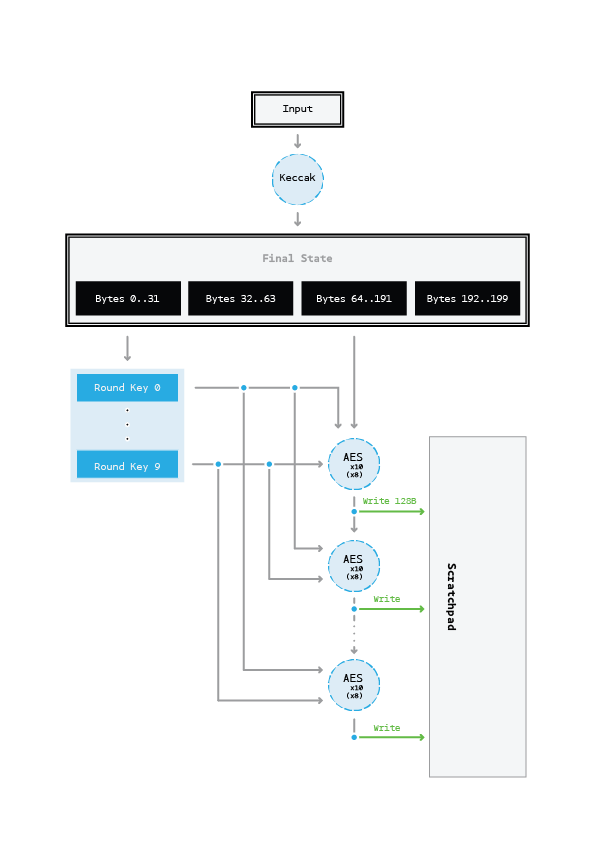
\includegraphics[scale=0.65,keepaspectratio]{Images/Bill/initialization.png}
  \caption{Scratchpad initialization.~\cite{bill}}
  \label{fig:initialization}
\end{figure}
\clearpage

\subsection{The second stage (memory-hardness)} \label{sec:second}
The second stage of the algorithm uses the initialized scratchpad and two values that are computed from the hashed input of the function. Its goal is to perform computations on the scratchpad values (on all of them with high probability) and produce a final scratchpad structure that can't be computed otherwise or in stages (without huge time complexity). The memory-hardness property is satisfied if and only if there is no other way to compute the final state of the scratchpad using less memory than the size of the scratchpad. That is the overview. Let's see the details.

\paragraph{(The preparation part)} The core structure of this stage is a loop. However, before illustrating the computations that take place inside the loop, there are some computations needed for preparation and two technical clarifications.

\begin{enumerate}
  \item \label{memh: step 1} Compute the values of $a$ and $b$.
\end{enumerate}
Elements $a$ and $b$ are the two values which, along with the scratchpad, are given as input to the loop. More specifically, the first 64 bytes of the hashed input (the Keccak state) are split in two parts (32 bytes each part) and XOR-ed ($\oplus$), and the resulting 32 bytes are used to initialize variables $a$ and $b$, 16 bytes each.

\begin{figure}
  \centering
  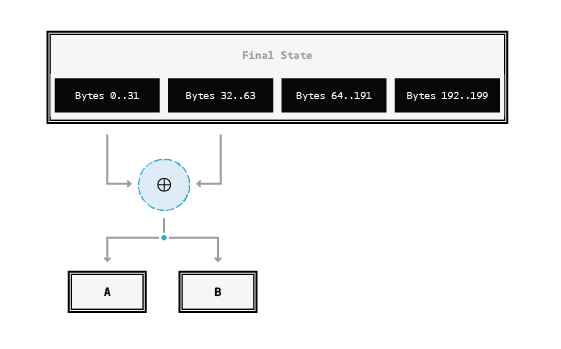
\includegraphics[scale=0.62,keepaspectratio]{Images/Bill/input_stage_2_modified.png}
  \caption{Extracting $a$ and $b$ values.~\cite{bill}}
  \label{fig:stage2input}
\end{figure}

In \hyperref[fig:stage2input]{figure}~\ref{fig:stage2input} the reader can see the visualization of this preparation part.
\clearpage

\begin{tcolorbox}[colback=yellow!5!white,colframe=yellow!65!black,title=\emph{Clarification 1:}]
  The reader may notice in \hyperref[fig:stage2]{figure}~\ref{fig:stage2} that the function uses a 16-byte value as an address in the scratchpad. Actually, the value is interpreted as a little-endian integer. The 21 low-order bits are used as a byte index. To ensure the 16-byte alignment, the four low-order bits of the index are cleared. This alignment is essential, as the data is read from and written to the scratchpad in 16-byte blocks.
\end{tcolorbox}
\vspace{0.2cm}

\begin{tcolorbox}[colback=yellow!5!white,colframe=yellow!65!black,title=\emph{Clarification 2:}]
  The main loop is iterated $524,288 = 2^{19}$ times. Every time, two blocks of the scratchpad are written, so with high probability, the whole scratchpad will be overwritten. In every iteration, along with the two blocks of the scratchpad, values $a'$ and $b'$ are computed, which are used as input to the next iteration.
\end{tcolorbox}
\vspace{0.2cm}

Now we are ready to describe the inner computations of the loop. We will divide this stage into parts, as it will help us later in the analysis. The number of parts are determined based on some intermediate values. We refer the reader to the graphical representation of this stage, presented in \hyperref[fig:stage2]{figure}~\ref{fig:stage2}.

Here, we note that the intermediate values are not memory requirements, as we can implement the computations with only 32 bytes of memory (for $a$ and $b$) plus the memory needed for the scratchpad. But during theoretical analysis and understanding of the function's computations, these intermediate values seem natural stops of the train of thought. So, after the \hyperref[memh: step 1]{step}~\ref{memh: step 1}:

\begin{enumerate}
  \setcounter{enumi}{1}
  \item \label{memh: step 2} Interpret the value of $a$ as a scratchpad address.
  \item \label{memh: step 3} Read from this address.
  \item Evaluate the AES function with data from \hyperref[memh: step 3]{step}~\ref{memh: step 3} and key the value of $a$.
\end{enumerate}
Let's call this intermediate value $c$. And let's add a final step to this part:
\begin{enumerate}
  \setcounter{enumi}{4}
  \item Calculate $c \oplus b$ and write the result to the address of \hyperref[memh: step 2]{step}~\ref{memh: step 2}.
\end{enumerate}
The value $c$ is passed as $b'$, part of the input of the next iteration. The second part involves another read from the scratchpad:

\begin{enumerate}
  \setcounter{enumi}{5}
  \item \label{memh: step 6} Interpret the value of $c$ as a scratchpad address.
  \item Read from this address. (We will refer to this intermediate value as $d$.)
  \item \label{memh: step 8} Multiply\footnote{The multiplication uses only the first 8 bytes of each argument, which are interpreted as unsigned 64-bit little-endian integers and multiplied together. The result is converted into 16 bytes, and finally the two 8-byte halves of the result are swapped~\cite{cryptonight}.} $c$, $d$ and add the value of $a$ to the result.
  \item Write the result of \hyperref[memh: step 8]{step}~\ref{memh: step 8} to the address of \hyperref[memh: step 6]{step}~\ref{memh: step 6}.
\end{enumerate}
This concludes the second part. The scratchpad is written twice per iteration. The only thing that is left to conclude the description of the second stage, is the computation of $a'$, part of the input of the next iteration. This is computed as follows:

\begin{enumerate}
  \setcounter{enumi}{9}
  \item Compute $d \oplus \mbox{(<the result of \hyperref[memh: step 8]{step}~\ref{memh: step 8}>) }$ to compute $a'$.
\end{enumerate}
\clearpage

\begin{figure}[H]
  \centering
  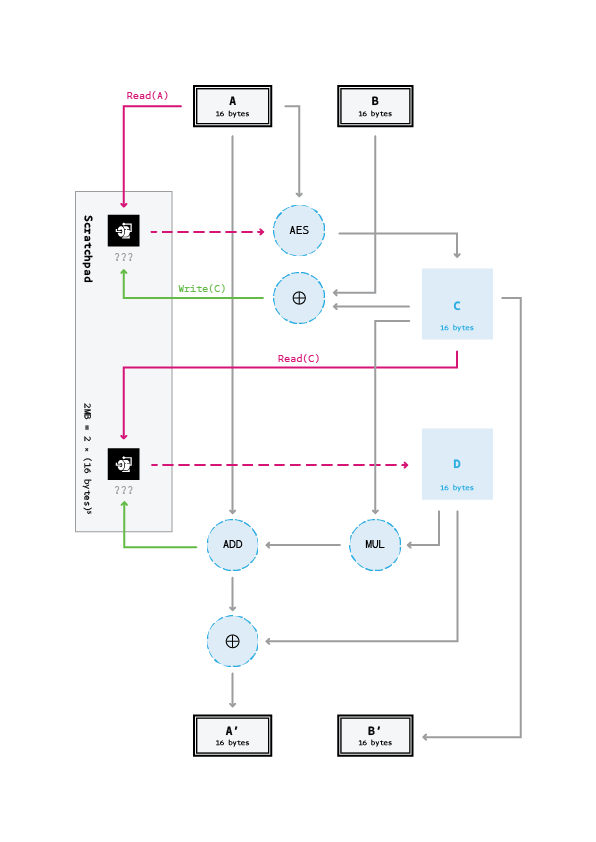
\includegraphics[scale=0.65,keepaspectratio]{Images/Bill/stage_2.png}
  \caption{The memory-hard part.~\cite{bill}}
  \label{fig:stage2}
\end{figure}

\subsection{The third stage}
The third stage of the algorithm uses the final state of the scratchpad to produce the output. During this stage AES operation is used. At first, the function extracts 10 key values from 32 bytes of the hashed input of the function, similar to the \hyperref[hashing]{step}~\ref{hashing} of the first stage. Extracting keys:
\begin{enumerate}
  \item Choose the bytes $[32...63]$ of the final Keccak state.
  \item Interpret them as an AES-256 key.
  \item \label{keys} Expand them to $10$ round keys.
\end{enumerate}
After this, the function needs a starting value. It applies XOR-operation($\oplus$) on bytes $[64...191]$ of the hashed input and the first 128 bytes of the scratchpad. Let's call these values \emph{input} and \emph{scratchpad[0]}.

\begin{enumerate}
  \setcounter{enumi}{3}
  \item \label{xor} \emph{input} $\oplus$ \emph{scratchpad[0]}.
\end{enumerate}
Now, using the first key of \hyperref[keys]{step}~\ref{keys} as key to the AES operation:

\begin{enumerate}
  \setcounter{enumi}{4}
  \item \label{encrypt} Encrypt the result of \hyperref[xor]{step}~\ref{xor}.
\end{enumerate}
Repeat the last two steps as follows:

\begin{itemize}
  \item Take the encrypted result of the last step as input.
  \item Take the next 128 bytes of the scratchpad (\emph{scratchpad[1]}).
  \item Use, as AES key, the next extracted key.
  \item Execute \hyperref[xor]{step}~\ref{xor} and \hyperref[encrypt]{step}~\ref{encrypt}.
\end{itemize}
until the last bytes of the scratchpad are used to the aforementioned operations. After the last bytes of the scratchpad are XOR-ed and encrypted,

\begin{enumerate}
  \setcounter{enumi}{5}
  \item \label{modified} Use the result to replace the bytes $[64...191]$ of the hashed input.
\end{enumerate}
We call the state of the hashed input after the above step as the \emph{modified Keccak state}. To produce the final result the function performs the next steps (see \hyperref[fig:stage3.1]{figure}~\ref{fig:stage3.2}).

\begin{enumerate}
  \setcounter{enumi}{5}
  \item Pass the \emph{modified Keccak state} through Keccak-$f$ (the Keccak permutation~\cite{keccak}).
  \item Choose the 2 low-order bits of the first byte of the \emph{modified Keccak state}.
  \item Based on these bits choose a hash function:
  \begin{align*}
     &\mbox{case 00: BLAKE-256} &
     &\mbox{case 01: Groestl-256}\\
     &\mbox{case 10: JH-256} &
     &\mbox{case 11: Skein-256}
  \end{align*}
  \item \label{output} Apply the chosen function to the \emph{modified Keccak state}.
\end{enumerate}
The result of \hyperref[output]{step}~\ref{output} is the output of the CryptoNight function. For more information about these functions, the reader is refered to the respective articles~\cite{10030667226,sha3groestl,sha3W09,sha3F+08}.

\begin{figure}[H]
  \centering
  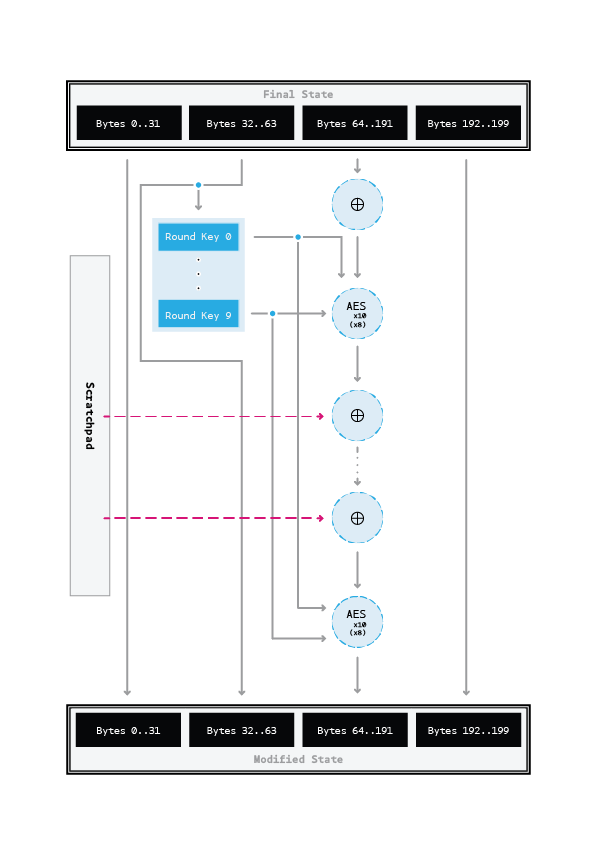
\includegraphics[scale=0.62, natwidth=210mm, natheight=297mm]{Images/Bill/stage_3.1.png}
  \caption{The third stage (1).~\cite{bill}}
  \label{fig:stage3.1}
\end{figure}
\clearpage

\begin{figure}[H]
  \centering
  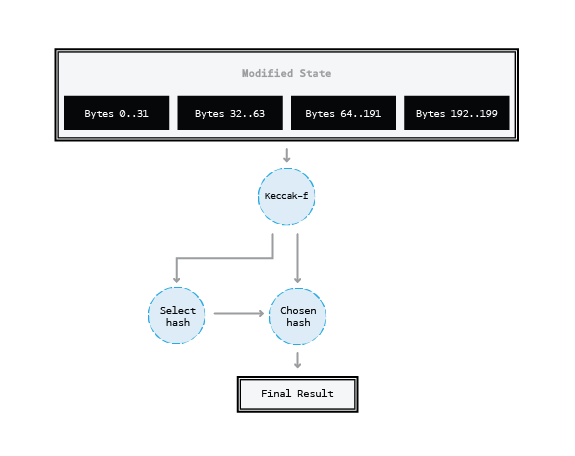
\includegraphics[scale=0.62, natwidth=210mm, natheight=148mm]{Images/Bill/stage_3.2_modified.png}
  \caption{The third stage (2).~\cite{bill}}
  \label{fig:stage3.2}
\end{figure}

\section{Analysis} \label{sec:analysis}
Now that we have described the way this function computes its output, we will try to build a model for our theoretical analysis. There are several assumptions that we have to make to abstract the function's operation. For this purpose, we build our model and define its security. At first, we have to focus on the part that is linked to the \hyperref[sec:memory-hard]{\emph{memory-hardness}} property (see \hyperref[sec:memory-hard]{section}~\ref{sec:memory-hard}). The reader now should have an understanding about the general purpose of each stage.

The first stage sets the scene for the memory-hardness part. We will assume that it initializes the scratchpad in a way, which is indistiguishable from the uniform distribution. It is safe to assume that, for an honest miner, the input is chosen uniformly at random as well. Our goal is to focus on the second stage, analyze it and then try to imagine, how an adversary miner can attack the memory-hardness property of this function. Due to the aforementioned assumptions we can conclude that the input of the second stage is chosen uniformly at random from its domain. Just to remember, the second stage's input is:
\begin{itemize}
  \item $a$
  \item $b$
  \item Scratchpad, from now on denoted as $SP$
\end{itemize}

\subsection{Parameters}
One of the first things that we need to do is to parametrize the input. We can't talk about complexity or security without the relative size between our objects or calculations. Moreover, this kind of analysis can help to generalize results and conclusions.

We will arbitrarily choose $n$ as symbol for the size of $a$ and fix everything else respectively. With that analysis in mind, we are fixing our language. Symbols:

\[
  \begin{array}{lcl}
    \mbox{Size of }a \mbox{: } & \: & n \\
    \mbox{Size of }b \mbox{: } & \: & n \\
    \mbox{Size of }SP \mbox{: } & \: & \beta_{n} = 2 \cdot 10^{6} \mbox{ bytes } \approx 2 \cdot n^{5} \mbox{ (polynomial)} \\
    \mbox{Value of }SP \mbox{ in address }x \mbox{: } & \: & SP_{x} \mbox{ (of size }n\mbox{)} \\
  \end{array}
\]

\subsection{AES as PRF}
The Advanced Encryption Standard (AES), also known by its original name Rijndael~\cite{Daemen99aesproposal:}, is a specification for the encryption of electronic data established by the U.S. National Institute of Standards and Technology (NIST) in 2001~\cite{nla.cat-vn4183631}.

AES is a subset of the Rijndael block cipher developed by two Belgian cryptographers, Vincent Rijmen and Joan Daemen, who submitted a proposal to NIST during the AES selection process. Rijndael is a family of ciphers with different key and block sizes.

For AES, NIST selected three members of the Rijndael family, each with a block size of 128 bits, but three different key lengths: 128, 192 and 256 bits.

AES has been adopted by the U.S. government and is now used worldwide. The algorithm described by AES is a symmetric-key algorithm, meaning the same key is used for both encrypting and decrypting the data.

In CryptoNight function AES is used for its properties as a cryptographic function. If a different key and a different input is chosen every time, then it is safe to assume that no prediction about the output of AES on this input can exist. To make this assumption more formal, we assume that AES is a \hyperref[sec:PRF]{pseudorandom function} (\hyperref[sec:PRF]{PRF}) and the seed is the key of AES.

In \hyperref[sec:PRF]{section}~\ref{sec:PRF} the reader can find the mathematical definition of PRFs. We define the notion and then we define a game. Based on this game we describe a security model to base the above assumption.

\subsection{Operations} \label{sec:operations}
Apart from the AES use, the memory-hard stage of CryptoNight function performs one addition, two XOR-operations and one multiplication. In order to be able to produce conclusions, we try to analyze what the side effects of these operations are. All of these operations get two inputs of 16 bytes size and produce a 16 byte result.

Let's examine them one by one. In the case of the XOR operation, it is easy to see that if the two inputs are chosen uniformly at random, then the result is also uniformly chosen at random. In the case of addition, reproduced from CryptoNote~\cite{cryptonight}:
\begin{verbatim}
   The 8byte_add function represents each of the arguments as a
   pair of 64-bit little-endian values and adds them together,
   component-wise, modulo 2^64. The result is converted back into
   16 bytes.
\end{verbatim}

It is trickier to see the same here, but with a little effort one can see that if the input is chosen uniformly at random, then the result is uniformly chosen at random too. In the case of multiplication, reproduced from CryptoNote~\cite{cryptonight} again:
\begin{verbatim}
   The 8byte_mul function, however, uses only the first 8 bytes
   of each argument, which are interpreted as unsigned 64-bit
   little-endian integers and multiplied together. The result is
   converted into 16 bytes, and finally the two 8-byte halves of
   the result are swapped.
\end{verbatim}

The last case, is more complex. At first we notice the following: if one of the inputs is null, then the result is also null. That could be a problem. We try to calculate the probability that the result is null, due to the null value of one or both inputs. We don't care about the null value of the result due to modulo operation. That probability is obviously equal to the probability that the result is equal with some other value. We would like the "extra" probability, that the value of the result is null due to input's null value, to be negligible.

Because of the special way CryptoNight function performs the multiplication, the inputs' sizes are 64 bits = 8 bytes = $\frac{n}{2}$. In addition, considering that AES is a PRF (assumption) and $SP$ is unifomly random (at least at the first round by assumption), then the two inputs are independent. The probability of one or both inputs to be null is:
\begin{equation} \label{prob_zero}
  \frac{1}{2^{n/2}} + \frac{1}{2^{n/2}} - \frac{1}{2^{n/2} \cdot 2^{n/2}} = \frac{2\cdot2^{n/2}-1}{2^n} < \frac{1}{2^{(n/2)-1}} = \mbox{\textbf{negl(n)}}
\end{equation}
\vspace{0.3cm}

That seems to be fine for our analysis. But, the next problem is this: Multiplication of two 8 byte numbers produces a result modulo 16 bytes (mod $2^{128}$). The reader can see that the probability of a value to be an output of the multiplication declines, as the values grow. Even after the swap that is performed at the end of the multiplication, the problem persists. We have not a uniformly at random distributed result, even if the inputs are chosen uniformly at random.

The above multiplication is perfomed this way because of the modern CPU registers' size. The 8 bytes multiplication is optimized. ASICs couldn't do this as fast as a modern CPU could, but technology advances and now there are chips that do the same computation roughly with the same time cost.

However, after our theoretical analysis we think that we should propose something better. The time cost of a 16 byte multiplication or maybe an 8 byte multiplication implementation that maps inputs' uniform distribution can make a system less efficient against ASICs, compared to the official implementation proposal, but not completely inefficient. Nevertheless, this is a detail and does not make great difference in our analysis. From now on, we can assume that the above problem is solved and we have a multiplication implementation that produces a uniformly at random distributed result.
